\section{Results \& discussion}
\label{sec:results}



\subsection{Baseline validation against exact dynamic programming}
\label{res:validation}

We compare baseline ADP with exact DP for $T=3$ and $\eta=13.75$. The exact fixed-threshold RU objective is $18.4911$, while the corresponding policy AVaR is $18.4900$, since $\eta$ is optimal only on the chosen grid.

Figure~\ref{fig:val-root} shows the estimated root RU objective against Bellman backups. At the largest budget, the mean estimate is $18.8607$ with standard deviation $0.0298$, giving an error of $0.3696$. The estimates become more stable across seeds but remain above the exact value, without monotone error reduction.

\begin{figure}[H]
	\centering
	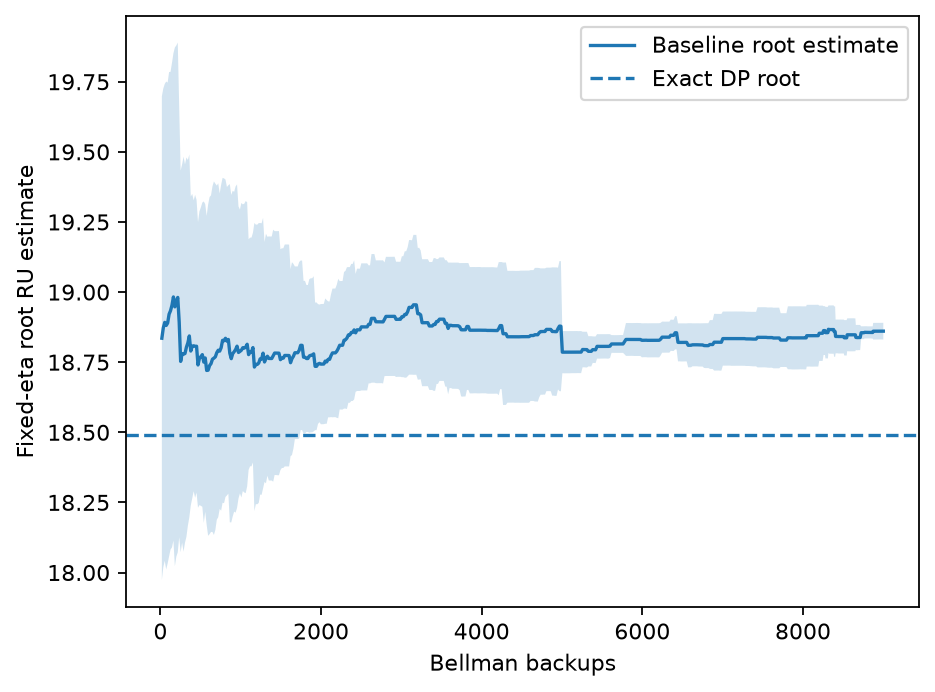
\includegraphics[width=0.78\textwidth]
	{figures/00_validation/root_convergence.png}
	\caption{Root RU estimates with training-seed standard deviations.}
	\label{fig:val-root}
\end{figure}

We evaluate policy quality on 2,000 shared disturbance trajectories. Table~\ref{tab:val} reports paired differences averaged over three training seeds. The root RU error is the mean absolute prediction error. The RU and AVaR gaps compare evaluated policies using the fixed threshold and empirical AVaR, respectively. Positive gaps favor exact DP.

\begin{table}[H]
	\centering
	\caption{Baseline errors relative to exact DP.}
	\label{tab:val}
	\begin{tabular}{rrrrr}
		\hline
		Backups &
		Root RU error &
		RU gap &
		AVaR gap &
		Mean-cost gap \\
		\hline
		900   & 0.4934 & 0.0065 & 0.0055 & 0.0114 \\
		1,800 & 0.2965 & 0.0191 & 0.0166 & 0.0074 \\
		2,700 & 0.4030 & 0.0145 & 0.0111 & 0.0035 \\
		3,600 & 0.3903 & 0.0201 & 0.0166 & 0.0111 \\
		5,400 & 0.3035 & 0.0065 & 0.0055 & 0.0114 \\
		7,200 & 0.3429 & 0.0065 & 0.0055 & 0.0114 \\
		8,998 & 0.3696 & 0.0065 & 0.0055 & 0.0114 \\
		\hline
	\end{tabular}
\end{table}

The backup counts are averaged across seeds. Policy gaps remain small at all budgets, with no clear improvement as the budget increases. In contrast, root-value errors are noticeably larger.

Paired evaluation is important: the exact policy has an empirical AVaR of $19.6384$ on the shared sample, compared with $18.4900$ under full path enumeration. Thus, direct comparison with the enumerated value would mix policy and Monte Carlo errors.

Figure~\ref{fig:val-policy} shows the paired policy gaps. All 95\% Monte Carlo intervals for RU differences include zero. However, baseline evaluation may depend on the order in which states are visited because of random initialization and caching. Therefore, these results should be interpreted with caution and do not establish equal policy performance.

\begin{figure}[H]
	\centering
	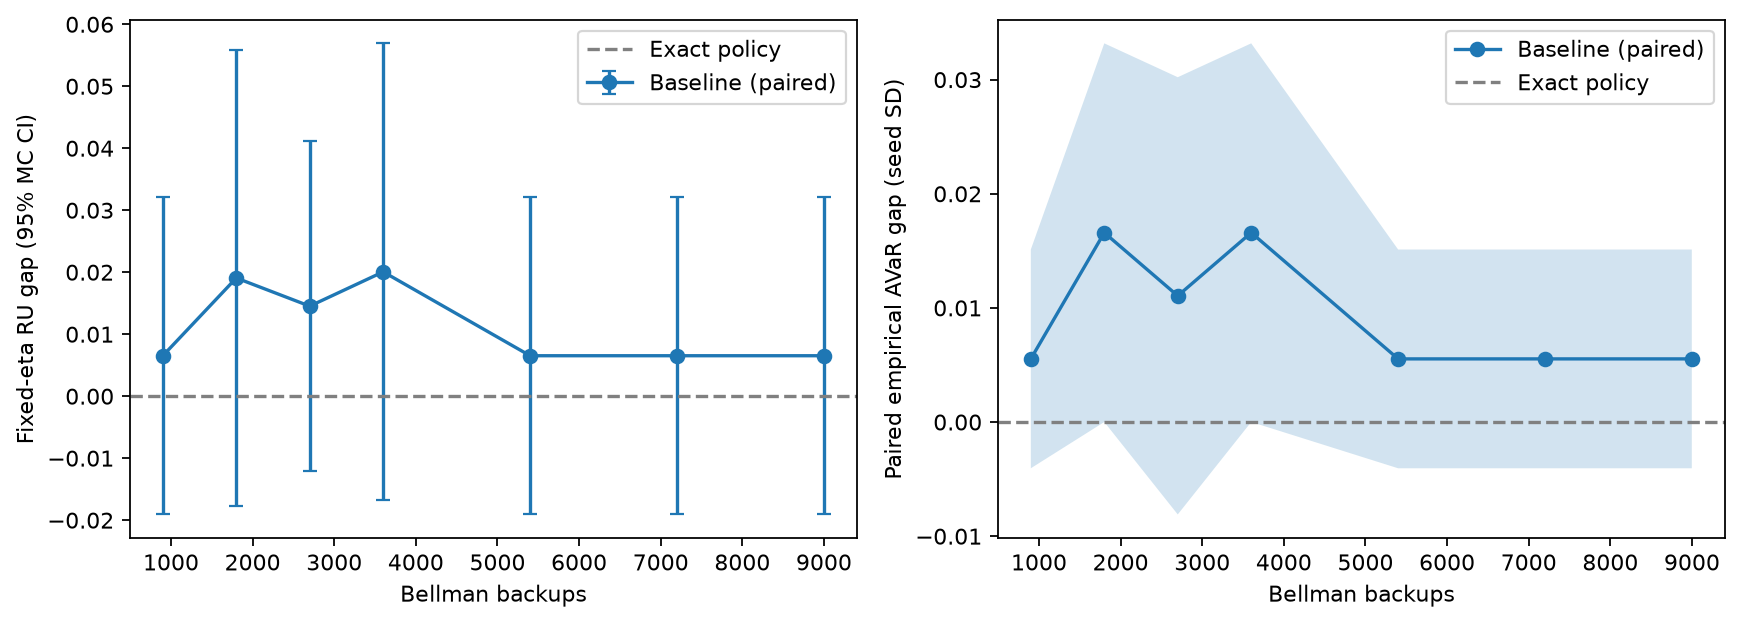
\includegraphics[width=\textwidth]
	{figures/00_validation/policy_performance.png}
	\caption{Paired policy gaps. Left: nominal 95\% Monte Carlo
		intervals. Right: training-seed standard deviations.}
	\label{fig:val-policy}
\end{figure}

The baseline also agrees with the exact policy at all 101 sampled test entries, for every seed and budget.

Overall, baseline ADP achieves policy performance close to exact DP despite noticeable root-value errors.

\subsection{Fixed-threshold probabilistic ADP}
\label{res:fixed}

We compare six probabilistic ADP sampling rules at $\eta=13.75$ for $T=3$ and $\eta=27.8325$ for $T=7$, evaluating policy quality across Bellman-backup budgets.

\paragraph{Empirical AVaR and RU objective.}

Figure~\ref{fig:fixed-risk} shows empirical AVaR and evaluated fixed-threshold RU objectives, both calculated from policy rollouts. For $T=3$, decision-aware sampling gives lower AVaR than random and uncertainty sampling at every budget. At 3,597 backups, the mean values are $19.7929$, $20.4940$, and $20.7308$, respectively. Decision-aware performance is already good at the smallest budget and changes little afterward.

For $T=7$, decision-aware AVaR decreases from $42.4413$ at 885 backups to $36.7091$ at 8,985 backups. At 3,585 backups, it achieves $36.8594$, compared with $40.4588$ for random and $52.4161$ for uncertainty sampling.

\begin{figure}[H]
	\centering
	\begin{subfigure}[b]{0.48\textwidth}
		\centering
		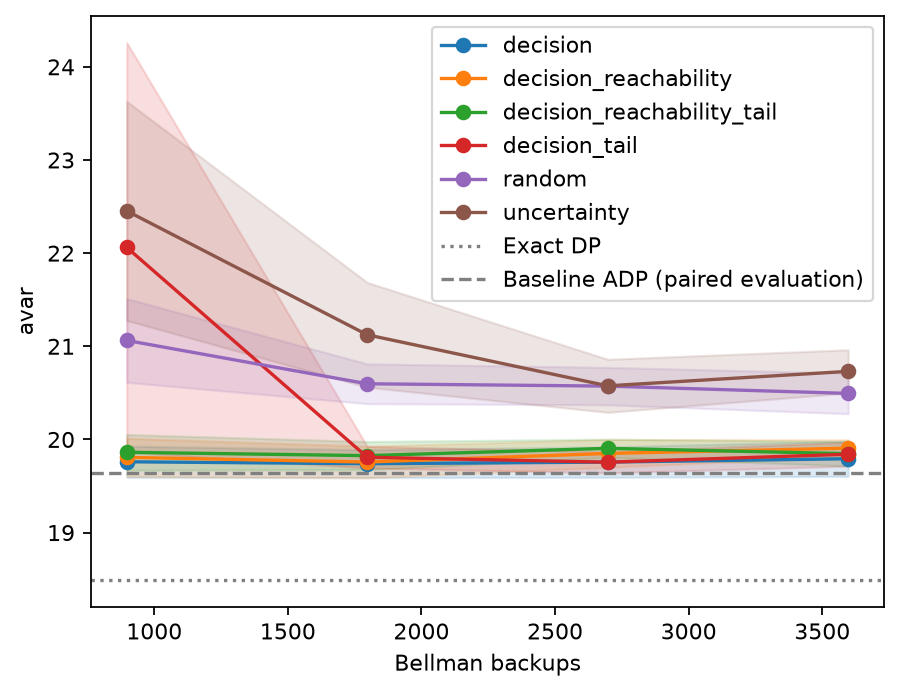
\includegraphics[width=\linewidth]{figures/01_fixed_eta/t3/avar_vs_backups.png}
		\caption{Empirical AVaR, $T=3$.}
		\label{fig:fixed-risk-avar-t3}
	\end{subfigure}
	\hfill
	\begin{subfigure}[b]{0.48\textwidth}
		\centering
		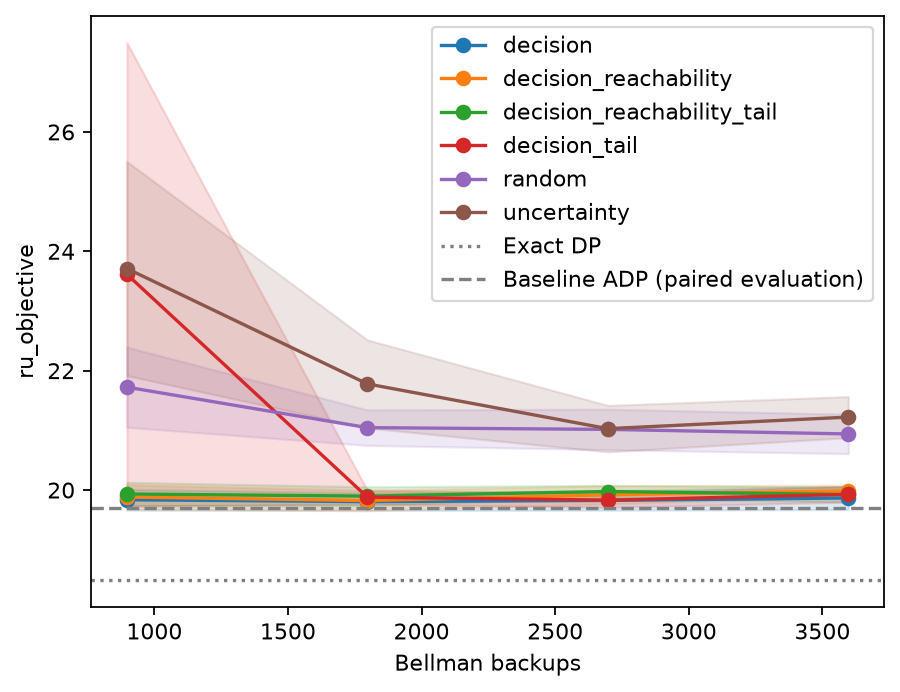
\includegraphics[width=\linewidth]{figures/01_fixed_eta/t3/ru_objective_vs_backups.png}
		\caption{Evaluated RU, $T=3$.}
		\label{fig:fixed-risk-ru-t3}
	\end{subfigure}
	
	\medskip
	
	\begin{subfigure}[b]{0.48\textwidth}
		\centering
		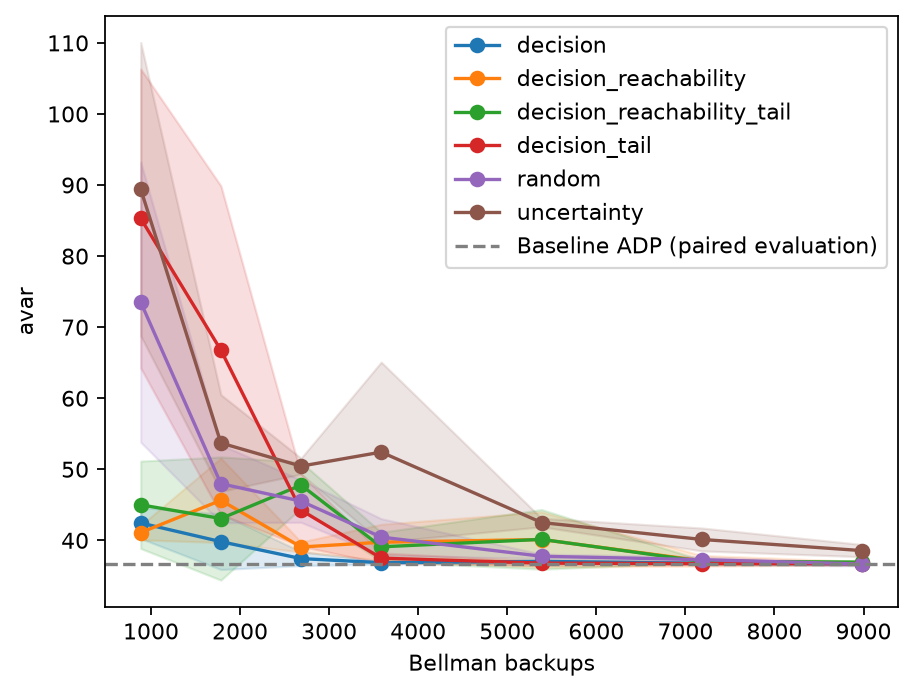
\includegraphics[width=\linewidth]{figures/01_fixed_eta/t7/avar_vs_backups.png}
		\caption{Empirical AVaR, $T=7$.}
		\label{fig:fixed-risk-avar-t7}
	\end{subfigure}
	\hfill
	\begin{subfigure}[b]{0.48\textwidth}
		\centering
		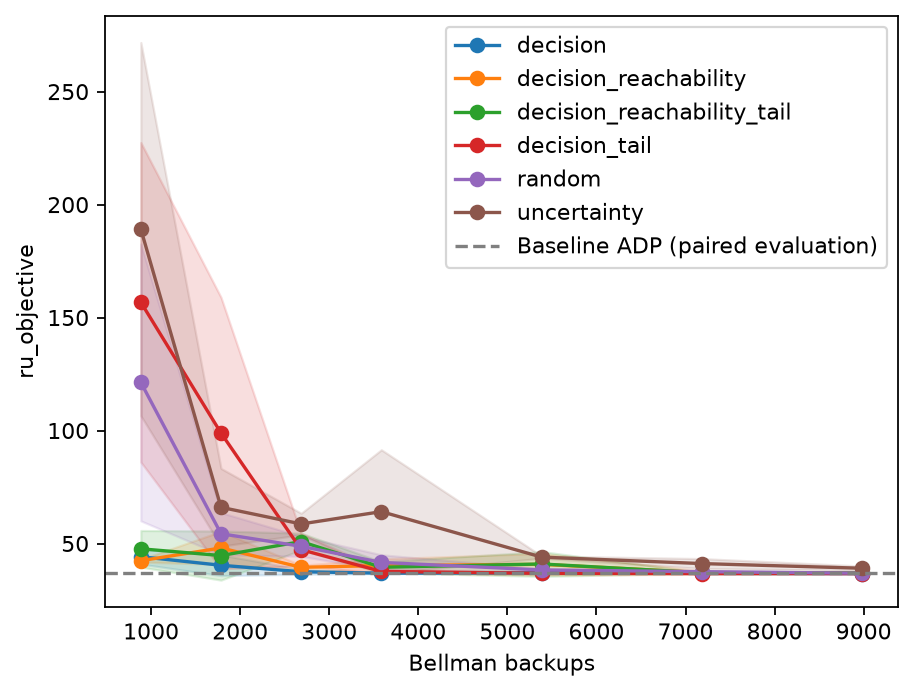
\includegraphics[width=\linewidth]{figures/01_fixed_eta/t7/ru_objective_vs_backups.png}
		\caption{Evaluated RU, $T=7$.}
		\label{fig:fixed-risk-ru-t7}
	\end{subfigure}
	
	\caption{Empirical AVaR and evaluated RU objective against Bellman backups. Shading shows training-seed standard deviations.}
	\label{fig:fixed-risk}
\end{figure}

\paragraph{Comparison with exact DP.}

For $T=3$, the exact policy has AVaR $18.4900$ under full enumeration, but $19.6384$ on the shared 2,000-trajectory evaluation sample. Thus, comparing GP results directly with the enumerated reference includes significant Monte Carlo error.

Figure~\ref{fig:fixed-exact} shows paired RU gaps against exact DP. At 3,597 backups, decision-aware sampling has a mean gap of $0.1704$, with approximate 95\% Monte Carlo interval $[-0.0137,0.3545]$. Random and uncertainty sampling give larger gaps of $1.2430$ and $1.5251$, with intervals above zero. All decision-aware intervals include zero, but this does not establish equality with the exact policy. The intervals measure Monte Carlo uncertainty after averaging across training seeds.

\begin{figure}[H]
	\centering
	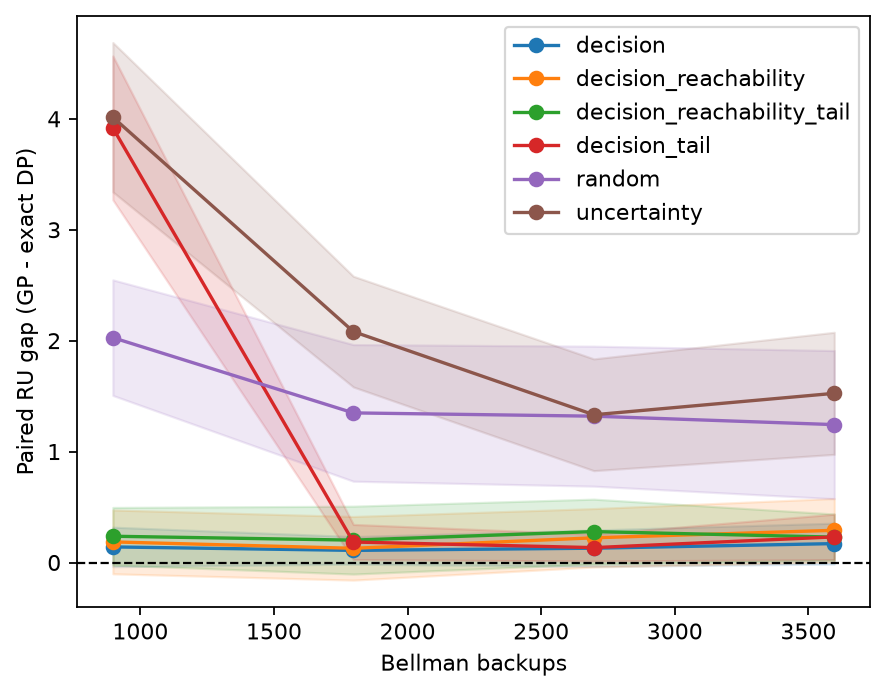
\includegraphics[width=0.78\textwidth]
	{figures/01_fixed_eta/t3/paired_exact_ru_vs_backups.png}
	\caption{Paired RU gaps against exact DP at $T=3$,
		with approximate 95\% Monte Carlo intervals.}
	\label{fig:fixed-exact}
\end{figure}

\paragraph{Comparison with baseline ADP.}

Table~\ref{tab:fixed-paired} reports paired differences against saved baseline policies at the largest budgets. Negative gaps favor probabilistic ADP. The reference uses three baseline policies for $T=3$ and one for $T=7$.

\begin{table}[H]
	\centering
	\caption{Paired gaps relative to baseline ADP.}
	\label{tab:fixed-paired}
	\begin{tabular}{lrrrr}
		\hline
		& \multicolumn{2}{c}{$T=3$: 3,597 backups}
		& \multicolumn{2}{c}{$T=7$: 8,985 backups} \\
		Method & AVaR gap & RU gap & AVaR gap & RU gap \\
		\hline
		Random
		& 0.8500 & 1.2365 & -0.0636 & 0.1058 \\
		Uncertainty
		& 1.0869 & 1.5186 & 1.8196 & 2.3121 \\
		Decision
		& 0.1489 & 0.1639 & -0.0255 & -0.0203 \\
		Decision + reachability
		& 0.2625 & 0.2837 & 0.0558 & 0.0553 \\
		Decision + tail
		& 0.1972 & 0.2242 & -0.0086 & -0.0082 \\
		Decision + reachability + tail
		& 0.2034 & 0.2223 & 0.2043 & 0.2037 \\
		\hline
	\end{tabular}
\end{table}

For $T=7$, decision-aware sampling approaches baseline performance by 3,585 backups. At the largest budget, its gaps are slightly negative but small relative to training-seed variation (standard deviations $0.2956$ for AVaR and $0.3051$ for RU). Random sampling gives a slightly lower empirical AVaR at this budget, but a higher RU objective and mean cost.

Figure~\ref{fig:fixed-paired} shows these comparisons across budgets. They remain descriptive because baseline evaluation can depend on randomized initialization and caching. The $T=7$ baseline is not an exact reference.

\begin{figure}[H]
	\centering
	\begin{subfigure}[b]{0.48\textwidth}
		\centering
		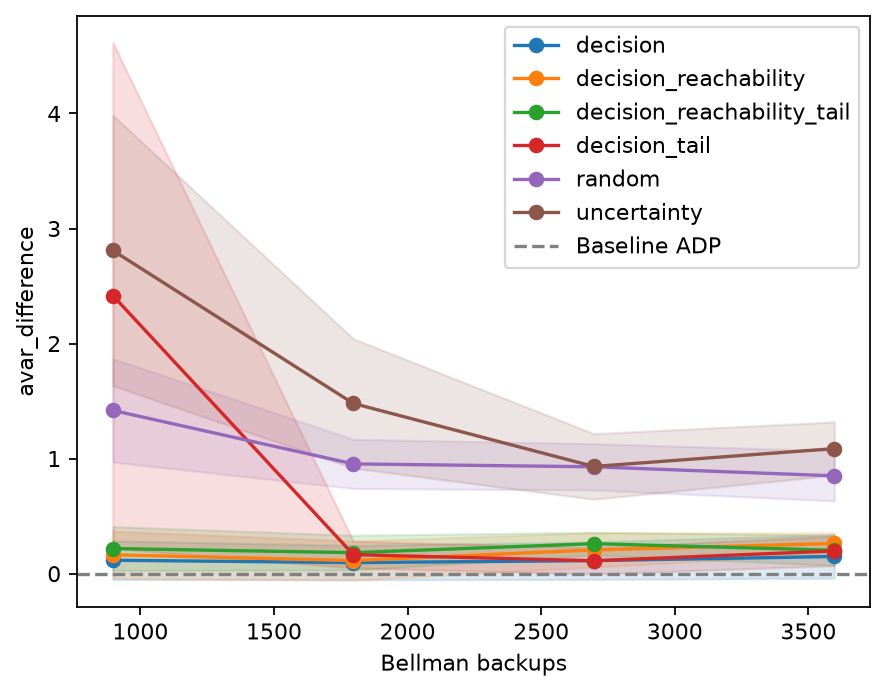
\includegraphics[width=\linewidth]{figures/01_fixed_eta/t3/paired_avar_difference_vs_backups.png}
		\caption{AVaR gaps, $T=3$.}
		\label{fig:fixed-paired-avar-t3}
	\end{subfigure}
	\hfill
	\begin{subfigure}[b]{0.48\textwidth}
		\centering
		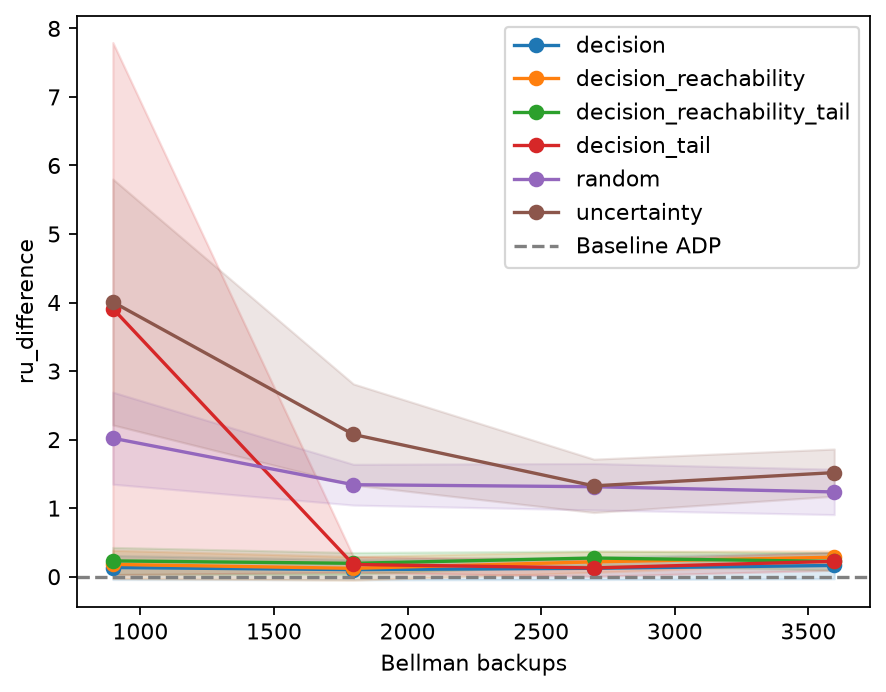
\includegraphics[width=\linewidth]{figures/01_fixed_eta/t3/paired_ru_difference_vs_backups.png}
		\caption{RU gaps, $T=3$.}
		\label{fig:fixed-paired-ru-t3}
	\end{subfigure}
	
	\medskip
	
	\begin{subfigure}[b]{0.48\textwidth}
		\centering
		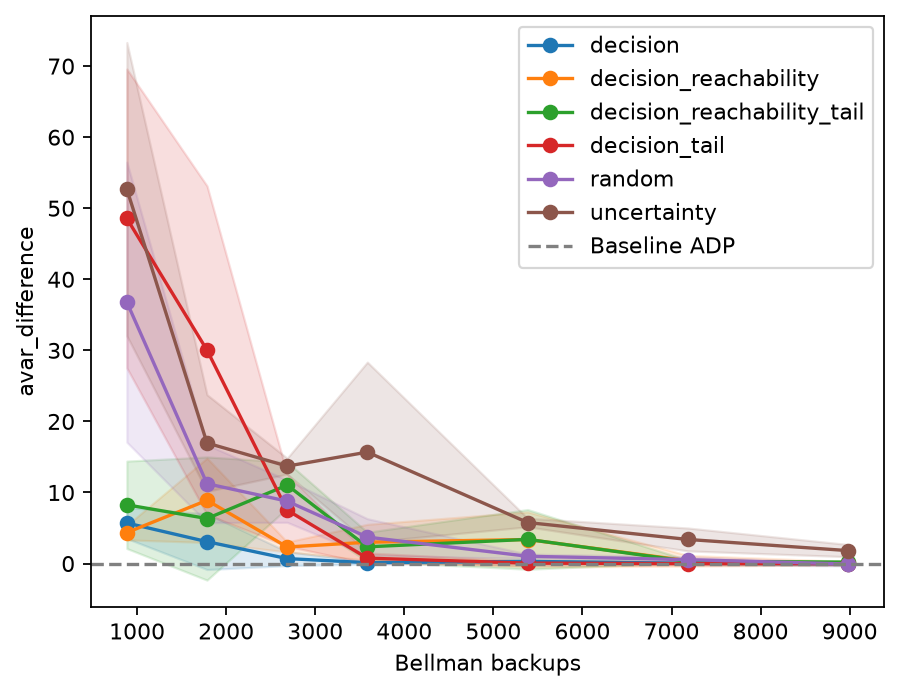
\includegraphics[width=\linewidth]{figures/01_fixed_eta/t7/paired_avar_difference_vs_backups.png}
		\caption{AVaR gaps, $T=7$.}
		\label{fig:fixed-paired-avar-t7}
	\end{subfigure}
	\hfill
	\begin{subfigure}[b]{0.48\textwidth}
		\centering
		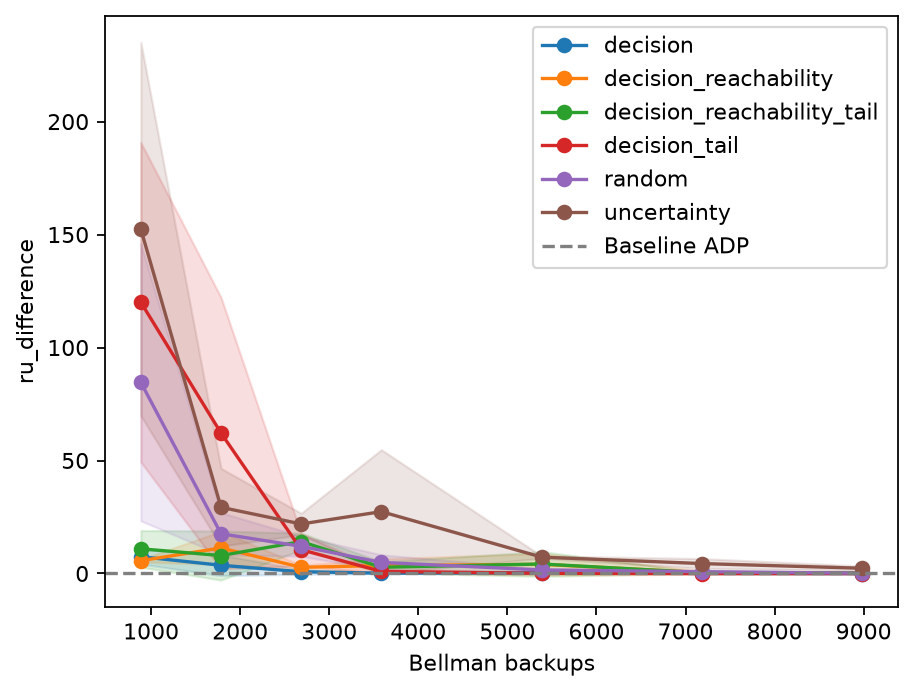
\includegraphics[width=\linewidth]{figures/01_fixed_eta/t7/paired_ru_difference_vs_backups.png}
		\caption{RU gaps, $T=7$.}
		\label{fig:fixed-paired-ru-t7}
	\end{subfigure}
	
	\caption{Paired AVaR and RU gaps to baseline ADP. Shading shows training-seed standard deviations.}
	\label{fig:fixed-paired}
\end{figure}

\paragraph{Acquisition rules and computational cost.}

Adding reachability or tail relevance does not consistently improve decision-aware sampling. Tail weighting is particularly unstable at small budgets, giving mean AVaR $85.2944$ for $T=7$ at 885 backups.

At $T=3$ and 3,597 backups, decision-aware sampling disagrees with the exact policy on only $4.46\%$ of sampled test entries, compared with $38.61\%$ for random and $40.10\%$ for uncertainty sampling.

Predicted objectives also differ from evaluated risk. For decision-aware sampling at $T=7$ and 8,985 backups, predicted and evaluated RU objectives are $38.6927$ and $36.7169$, respectively.

The saved baselines use approximately 18,000 training backups for $T=3$ and 41,766 for $T=7$. Decision-aware GP sampling achieves comparable policy performance with substantially fewer backups and lower recorded training times in these runs. However, this does not establish general speedup factors or the minimum baseline budget needed.

Within probabilistic ADP, active sampling has additional computational costs. At 8,985 backups and $T=7$, decision-aware training takes about 243 seconds, compared with 60 seconds for random sampling. Thus, backup efficiency does not necessarily imply runtime efficiency.

\subsection{Outer-threshold optimization}
\label{res:outer}

We compare random, uncertainty, and decision-aware sampling over $\mathcal{H}=\{0,0.25,\dots,40\}$, using one collection of GP models for all thresholds. The threshold minimizing the predicted RU objective is selected, and its policy is evaluated over shared trajectories.

The outer search requires 483 root backups. At the smallest budget of 897 backups, only 414 remain for GP training.

\paragraph{Selected thresholds.}

Figure~\ref{fig:outer-eta} shows the selected thresholds. At 8,997 backups, decision-aware sampling gives mean $\hat{\eta}=13.525$ for $T=3$, close to the exact grid-optimal value $13.75$. For $T=7$, it gives $\hat{\eta}=27.850$, close to the heuristic pilot value $27.8325$. Neither agreement establishes optimality beyond the available reference.

One random-sampling run at the smallest $T=7$ budget selects the upper boundary $\eta=40$, indicating a possible limitation of the search interval.

\begin{figure}[H]
	\centering
	\begin{subfigure}[b]{0.48\textwidth}
		\centering
		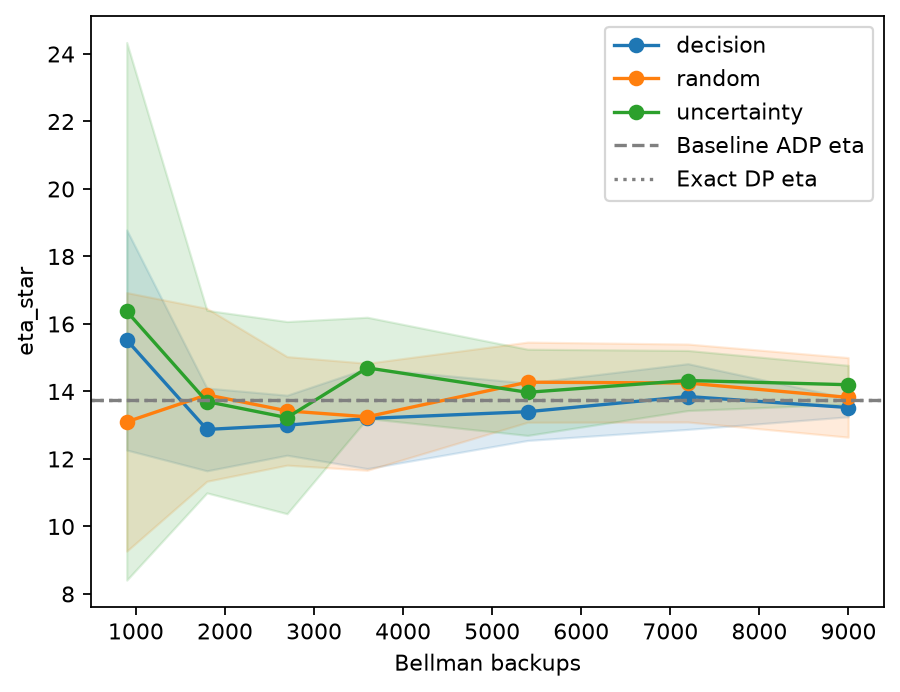
\includegraphics[width=\linewidth]{figures/02_outer_eta/t3/eta_vs_backups.png}
		\caption{Selected thresholds, $T=3$.}
		\label{fig:outer-eta-t3}
	\end{subfigure}
	\hfill
	\begin{subfigure}[b]{0.48\textwidth}
		\centering
		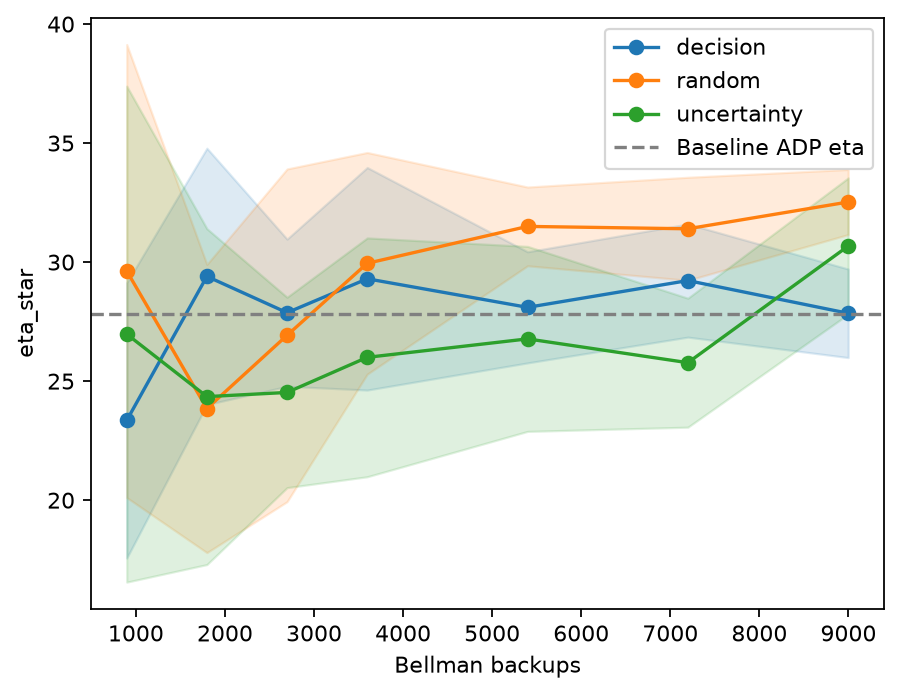
\includegraphics[width=\linewidth]{figures/02_outer_eta/t7/eta_vs_backups.png}
		\caption{Selected thresholds, $T=7$.}
		\label{fig:outer-eta-t7}
	\end{subfigure}
	
	\caption{Selected thresholds against Bellman backups. Shading shows training-seed standard deviations.}
	\label{fig:outer-eta}
\end{figure}

\paragraph{Predicted and evaluated objectives.}

Figure~\ref{fig:outer-ru} compares predicted minimum RU objectives with those evaluated from policy rollouts. After GP training, predictions require only root Bellman evaluations, without Monte Carlo policy rollouts. Their cost is independent of the evaluation sample size.

However, predictions are not always accurate. For $T=3$ at 897 backups, random sampling predicts $17.8852$, below the exact grid minimum $18.4911$, while its evaluated RU is $28.3359$. At the largest budget, decision-aware sampling gives predicted and evaluated RU values of $18.8761$ and $20.1483$ for $T=3$, and $38.3366$ and $36.7794$ for $T=7$. These differences reflect both approximation and Monte Carlo evaluation errors, which are not separated in this experiment.

\begin{figure}[H]
	\centering
	\begin{subfigure}[b]{\textwidth}
		\centering
		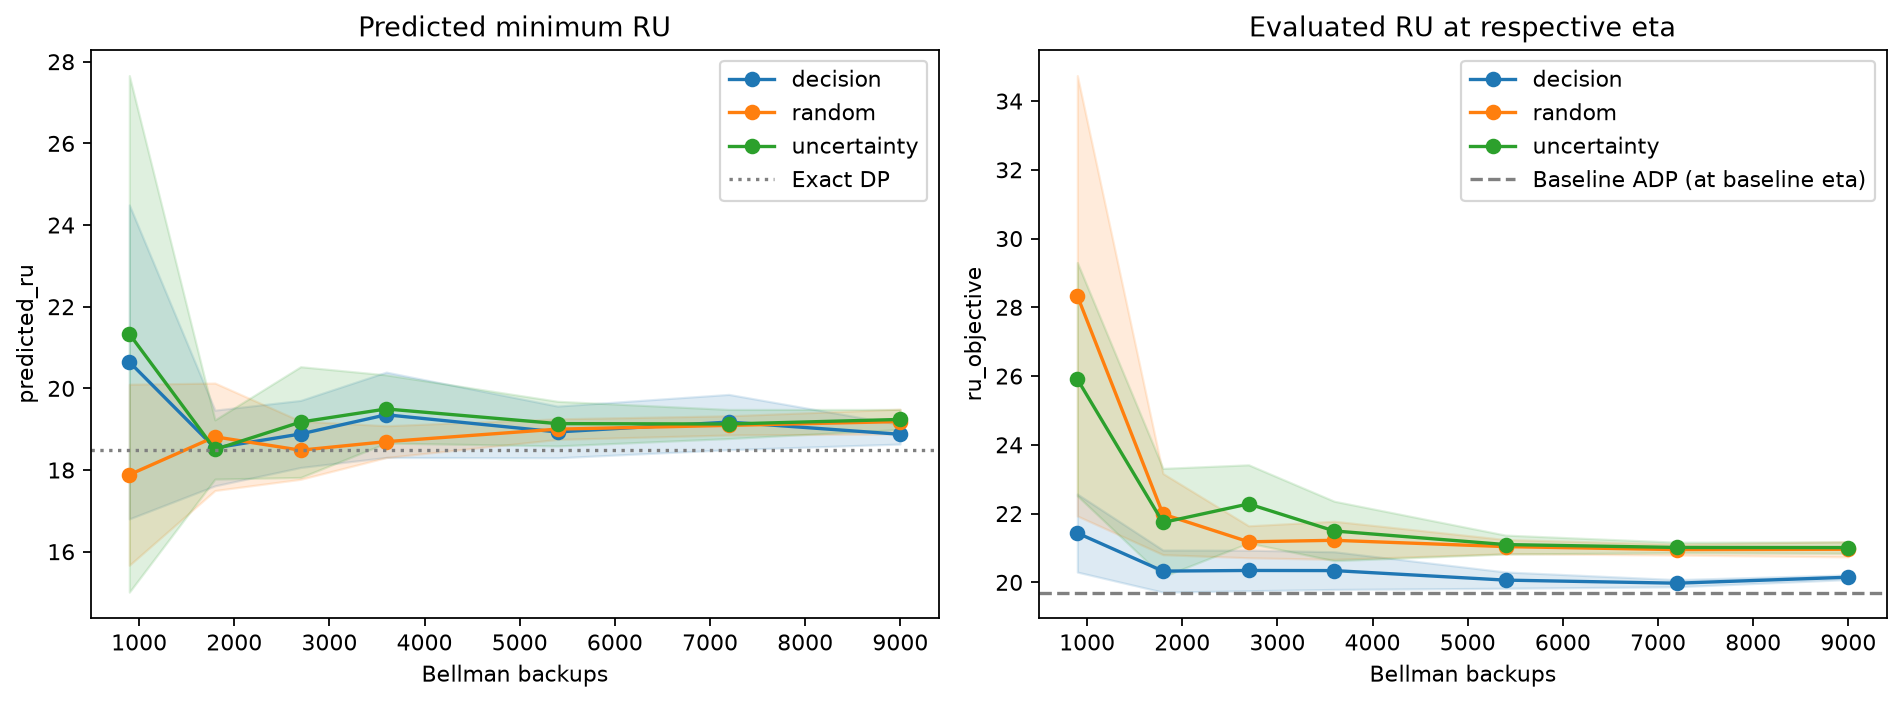
\includegraphics[width=\linewidth]{figures/02_outer_eta/t3/ru_vs_backups.png}
		\caption{Predicted minimum and evaluated RU, $T=3$.}
		\label{fig:outer-ru-t3}
	\end{subfigure}
	
	\medskip
	
	\begin{subfigure}[b]{\textwidth}
		\centering
		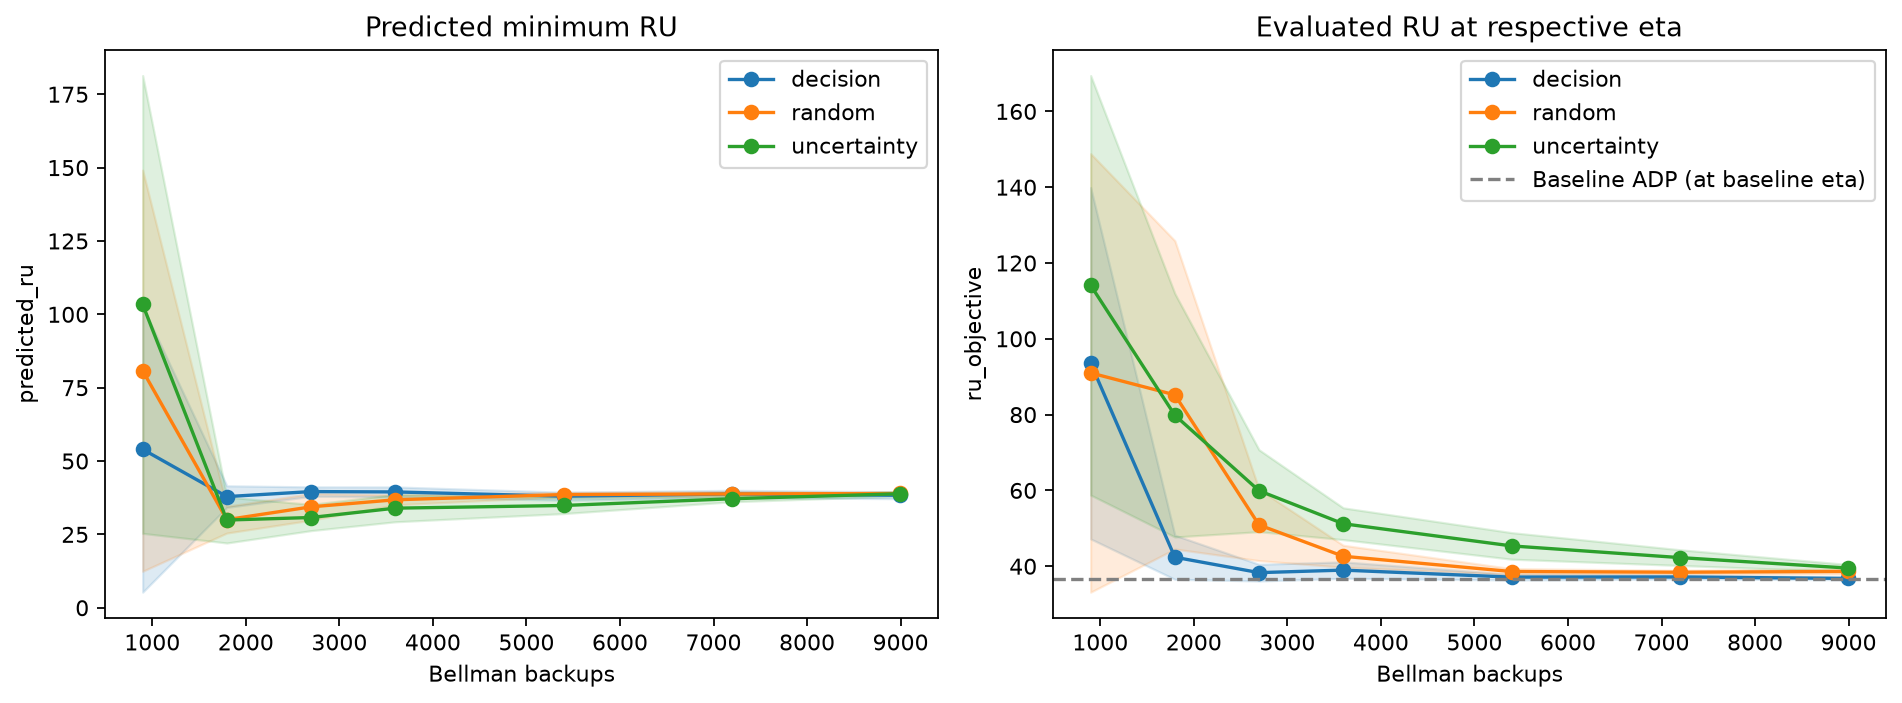
\includegraphics[width=\linewidth]{figures/02_outer_eta/t7/ru_vs_backups.png}
		\caption{Predicted minimum and evaluated RU, $T=7$.}
		\label{fig:outer-ru-t7}
	\end{subfigure}
	
	\caption{Predicted minimum RU (left) and evaluated RU (right) against Bellman backups. Shading shows training-seed standard deviations.}
	\label{fig:outer-ru}
\end{figure}

\paragraph{Evaluated policy performance.}

Table~\ref{tab:outer} reports the results at the largest budget. Decision-aware sampling achieves the lowest mean empirical AVaR and mean cost for both horizons. For $T=7$, its AVaR decreases from $57.2183$ at 897 backups to $36.5893$ at 8,997 backups. The improvement is less consistent for $T=3$.

\begin{table}[H]
	\centering
	\caption{Outer-threshold results at 8,997 backups.
		Means across ten training seeds.}
	\label{tab:outer}
	\begin{tabular}{llrrrr}
		\hline
		$T$ & Method & $\hat{\eta}$ & AVaR & Evaluated RU
		& Mean cost \\
		\hline
		\multirow{3}{*}{3} & Random      & 13.825 & 20.4978 & 20.9621 & 7.4354 \\
		 & Uncertainty & 14.200 & 20.6727 & 21.0112 & 7.5685 \\
		 & Decision    & 13.525 & 19.9907 & 20.1483 & 6.6625 \\
		\hline
		\multirow{3}{*}{7} & Random      & 32.525 & 38.1217 & 38.6228 & 16.1180 \\
		 & Uncertainty & 30.675 & 39.1253 & 39.5088 & 16.7823 \\
		 & Decision    & 27.850 & 36.5893 & 36.7794 & 14.7408 \\
		\hline
	\end{tabular}
\end{table}

\paragraph{Paired evaluation.}

Figure~\ref{fig:outer-paired} compares empirical AVaR against one saved fixed-threshold baseline policy per horizon, using shared disturbance trajectories.

At the largest budget, decision-aware sampling gives mean paired AVaR gaps of $0.3523$ for $T=3$ and $-0.1454$ for $T=7$. The latter has training-seed standard deviation $0.3136$, so it does not establish superiority over the baseline. Random and uncertainty sampling give larger gaps of $1.3871$ and $2.3906$ for $T=7$.

\begin{figure}[H]
	\centering
	\begin{subfigure}[b]{0.48\textwidth}
		\centering
		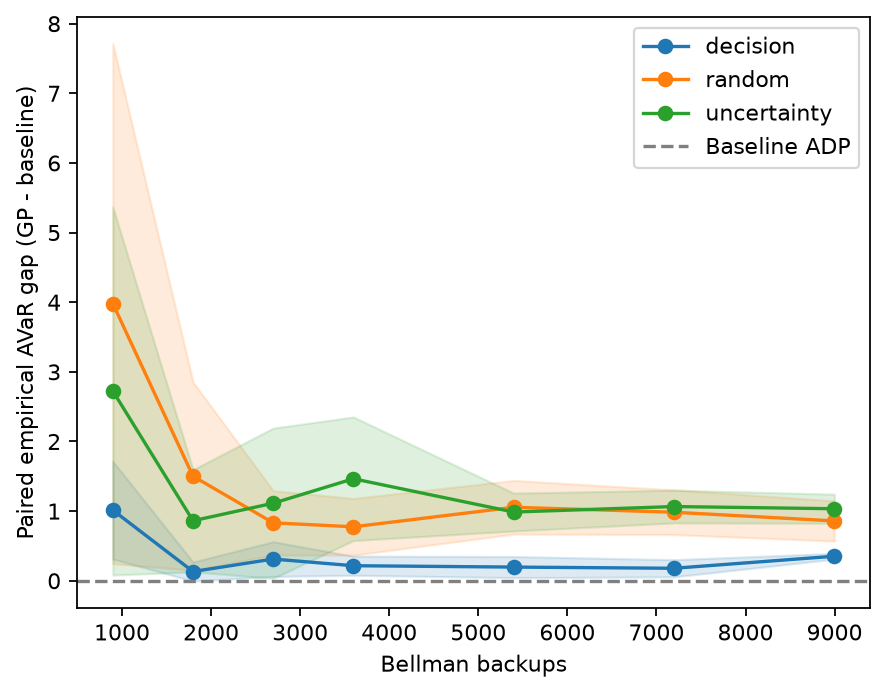
\includegraphics[width=\linewidth]{figures/02_outer_eta/t3/paired_avar_vs_backups.png}
		\caption{Paired AVaR gaps, $T=3$.}
		\label{fig:outer-paired-t3}
	\end{subfigure}
	\hfill
	\begin{subfigure}[b]{0.48\textwidth}
		\centering
		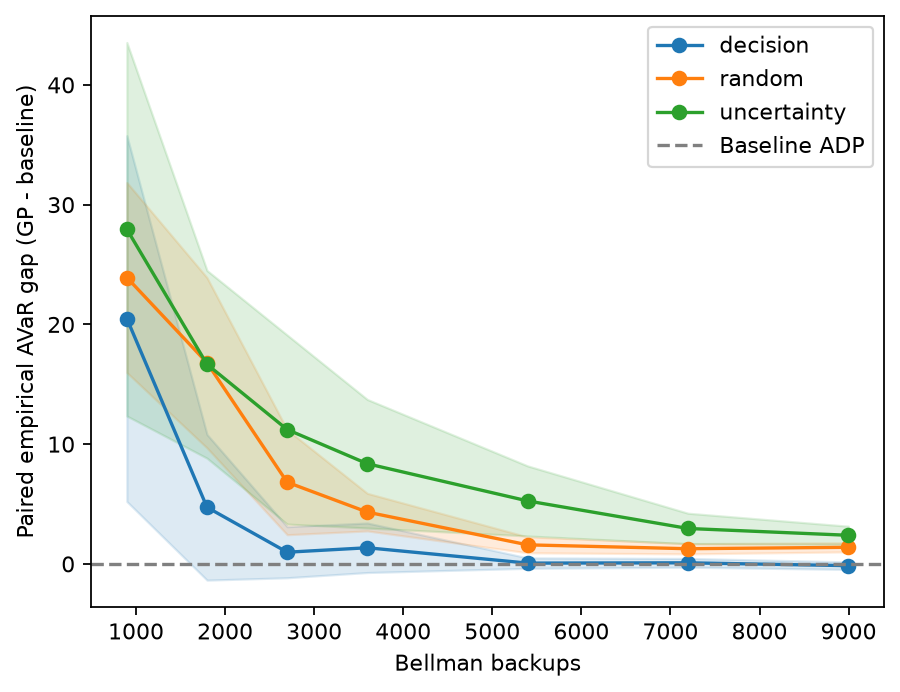
\includegraphics[width=\linewidth]{figures/02_outer_eta/t7/paired_avar_vs_backups.png}
		\caption{Paired AVaR gaps, $T=7$.}
		\label{fig:outer-paired-t7}
	\end{subfigure}
	
	\caption{Paired empirical AVaR gaps to baseline ADP against Bellman backups. Shading shows training-seed standard deviations.}
	\label{fig:outer-paired}
\end{figure}

We also compare RU gaps using the baseline threshold and each policy's own threshold, without changing the policies. For decision-aware sampling at $T=7$ and 8,997 backups, the gaps are $-0.1437$ and $0.0421$, with nominal 95\% Monte Carlo intervals $[-0.8676,0.5803]$ and $[-0.6857,0.7700]$, respectively. Both differences are small relative to their uncertainty, but baseline evaluation may depend on evaluation order. These results also show that the selected threshold does not always minimize the empirical RU objective.

\paragraph{Interpretation and computational cost.}

Decision-aware sampling gives better threshold and policy estimates than the other sampling methods in these experiments. However, we cannot conclude that outer optimization is better than fixed-threshold training, since the experiments use different candidate domains, budgets, and numbers of seeds.

Decision-aware sampling is also slower than random sampling. At the largest budget, mean training times are about 2,219 versus 98 seconds for $T=3$, and 412 versus 100 seconds for $T=7$. The higher runtime for $T=3$ may be explained by the larger number of training points per GP, since the backup budget is distributed across fewer stages. As GP fitting has roughly cubic complexity, training can be slower for shorter horizons despite having fewer stages.


\subsection{Candidate-pool ablation}
\label{res:pool}

We compare random and decision-aware sampling with 1,000 to 5,000 candidates per stage. Smaller pools are subsets of the same 5,000-point pool, with other training settings fixed. We use three training seeds and 20,000 shared evaluation trajectories. Due to different evaluation sample sizes, raw AVaR estimates are not directly compared with earlier experiments.

\paragraph{Effect on decision-aware sampling.}

Figure~\ref{fig:pool-decision} shows empirical AVaR across budgets. For $T=3$, larger pools generally improve performance. At 3,597 backups, increasing the pool from 1,000 to 5,000 candidates reduces mean AVaR from $19.4200$ to $18.8939$ and sampled policy disagreement from $32.01\%$ to $4.62\%$.

For $T=7$, the differences between pool sizes become small as the budget increases. At 8,985 backups, all methods give similar AVaR values, with no clear advantage from larger candidate pools. This suggests that pool size has little effect on policy performance at larger budgets.

\begin{figure}[H]
	\centering
	\begin{subfigure}[b]{0.48\textwidth}
		\centering
		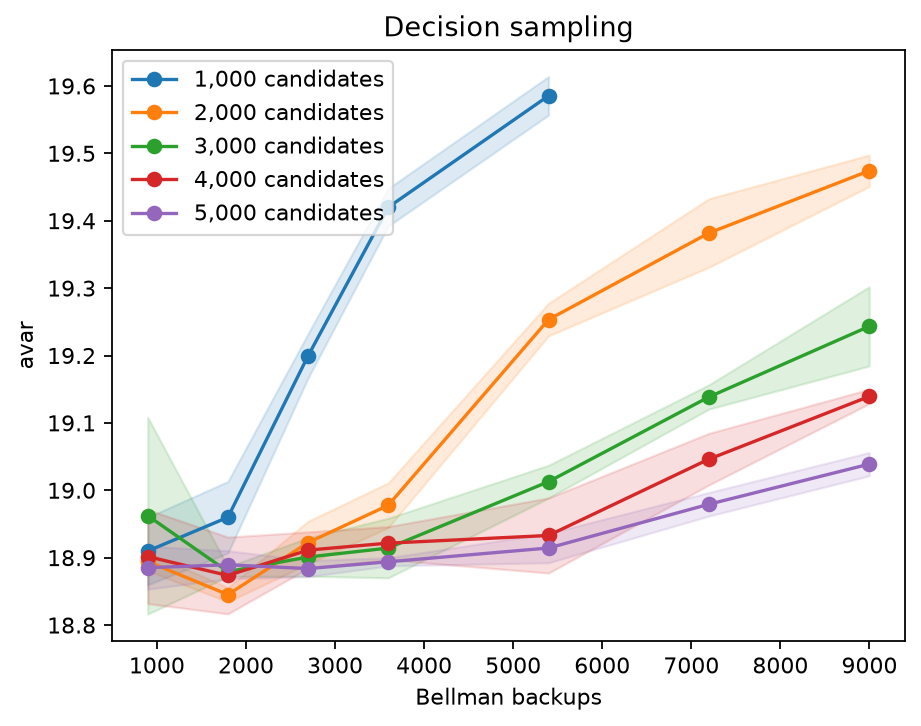
\includegraphics[width=\linewidth]{figures/03_candidate_pool/t3/avar_vs_backups_decision.png}
		\caption{Decision-aware AVaR, $T=3$.}
		\label{fig:pool-decision-t3}
	\end{subfigure}
	\hfill
	\begin{subfigure}[b]{0.48\textwidth}
		\centering
		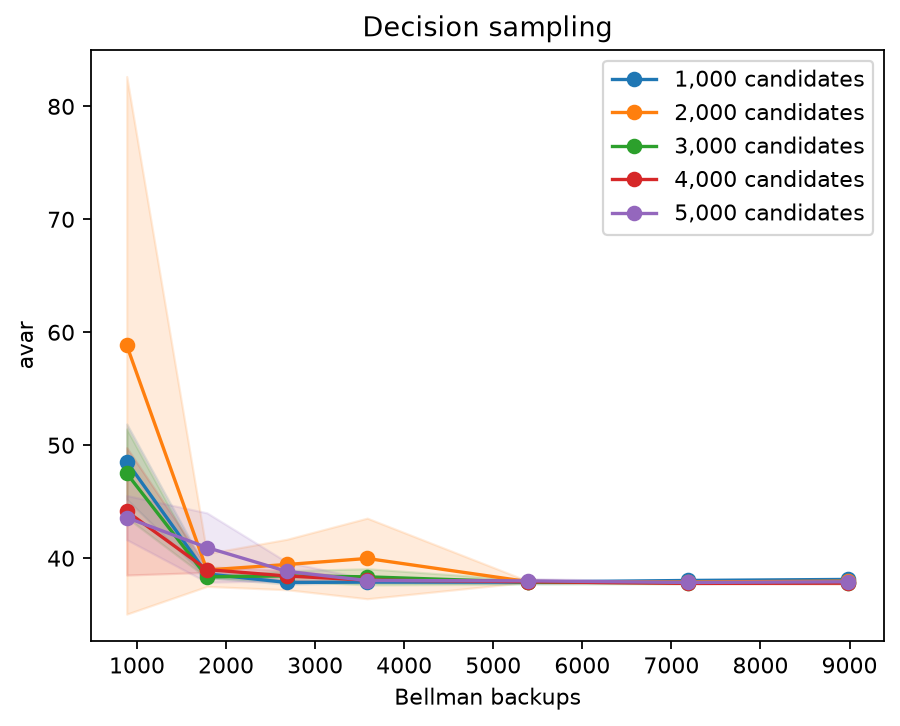
\includegraphics[width=\linewidth]{figures/03_candidate_pool/t7/avar_vs_backups_decision.png}
		\caption{Decision-aware AVaR, $T=7$.}
		\label{fig:pool-decision-t7}
	\end{subfigure}
	
	\caption{Decision-aware AVaR for different pool sizes. Shading shows training-seed standard deviations.}
	\label{fig:pool-decision}
\end{figure}

Table~\ref{tab:pool} summarizes the results at the nominal budget of 3,600 backups.

\begin{table}[H]
	\centering
	\caption{Decision-aware sampling at 3,600 nominal backups.}
	\label{tab:pool}
	\begin{tabular}{rrrr}
		\hline
		Candidates per stage &
		$T=3$ AVaR &
		$T=3$ disagreement (\%) &
		$T=7$ AVaR \\
		\hline
		1,000 & 19.4200 & 32.01 & 37.8834 \\
		2,000 & 18.9777 & 13.20 & 39.9740 \\
		3,000 & 18.9143 &  8.25 & 38.3482 \\
		4,000 & 18.9216 &  7.59 & 38.0603 \\
		5,000 & 18.8939 &  4.62 & 38.0193 \\
		\hline
	\end{tabular}
\end{table}

\paragraph{Paired comparisons between pool sizes.}

Figure~\ref{fig:pool-paired} shows paired empirical AVaR differences relative to the 5,000-point pool, using the same seeds, budgets, and disturbance paths. Positive differences favor the larger pool.

For decision-aware sampling at $T=3$, smaller pools become less effective at larger budgets. At 3,597 backups, the 1,000-point pool has a mean AVaR gap of $0.5261$, with training-seed standard deviation $0.0239$. Random sampling shows no similarly clear ordering, since it does not rank candidates by acquisition scores.

For $T=7$, differences between pools become small at larger budgets. With only three training seeds, the experiment does not establish a reliable ranking of pool sizes.

\begin{figure}[H]
	\centering
	\begin{subfigure}[b]{\textwidth}
		\centering
		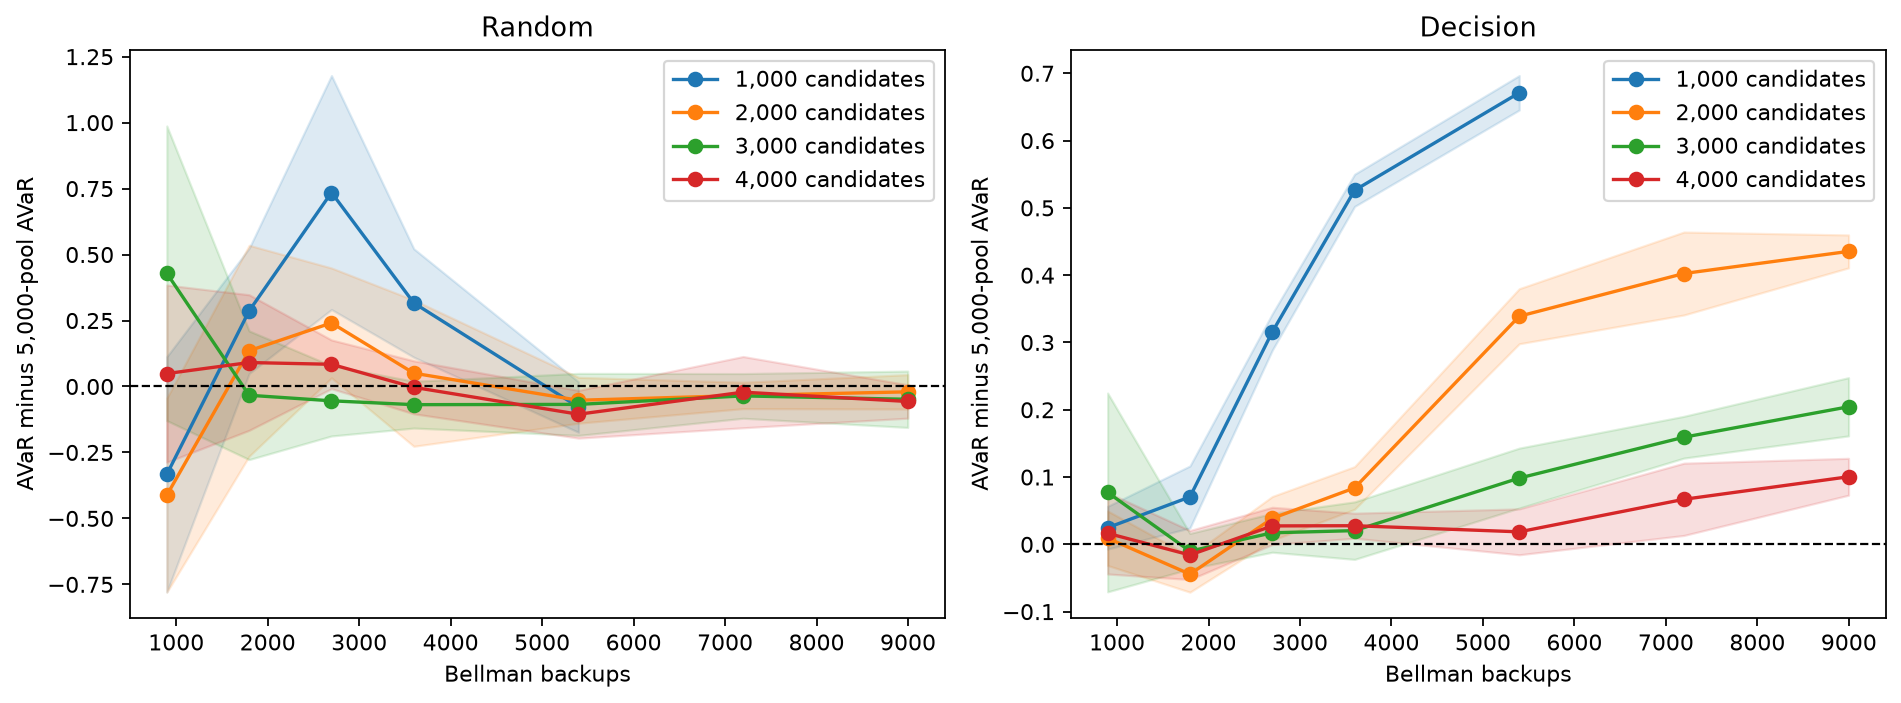
\includegraphics[width=\linewidth]{figures/03_candidate_pool/t3/avar_difference.png}
		\caption{Paired AVaR gaps, $T=3$.}
		\label{fig:pool-paired-t3}
	\end{subfigure}
	
	\medskip
	
	\begin{subfigure}[b]{\textwidth}
		\centering
		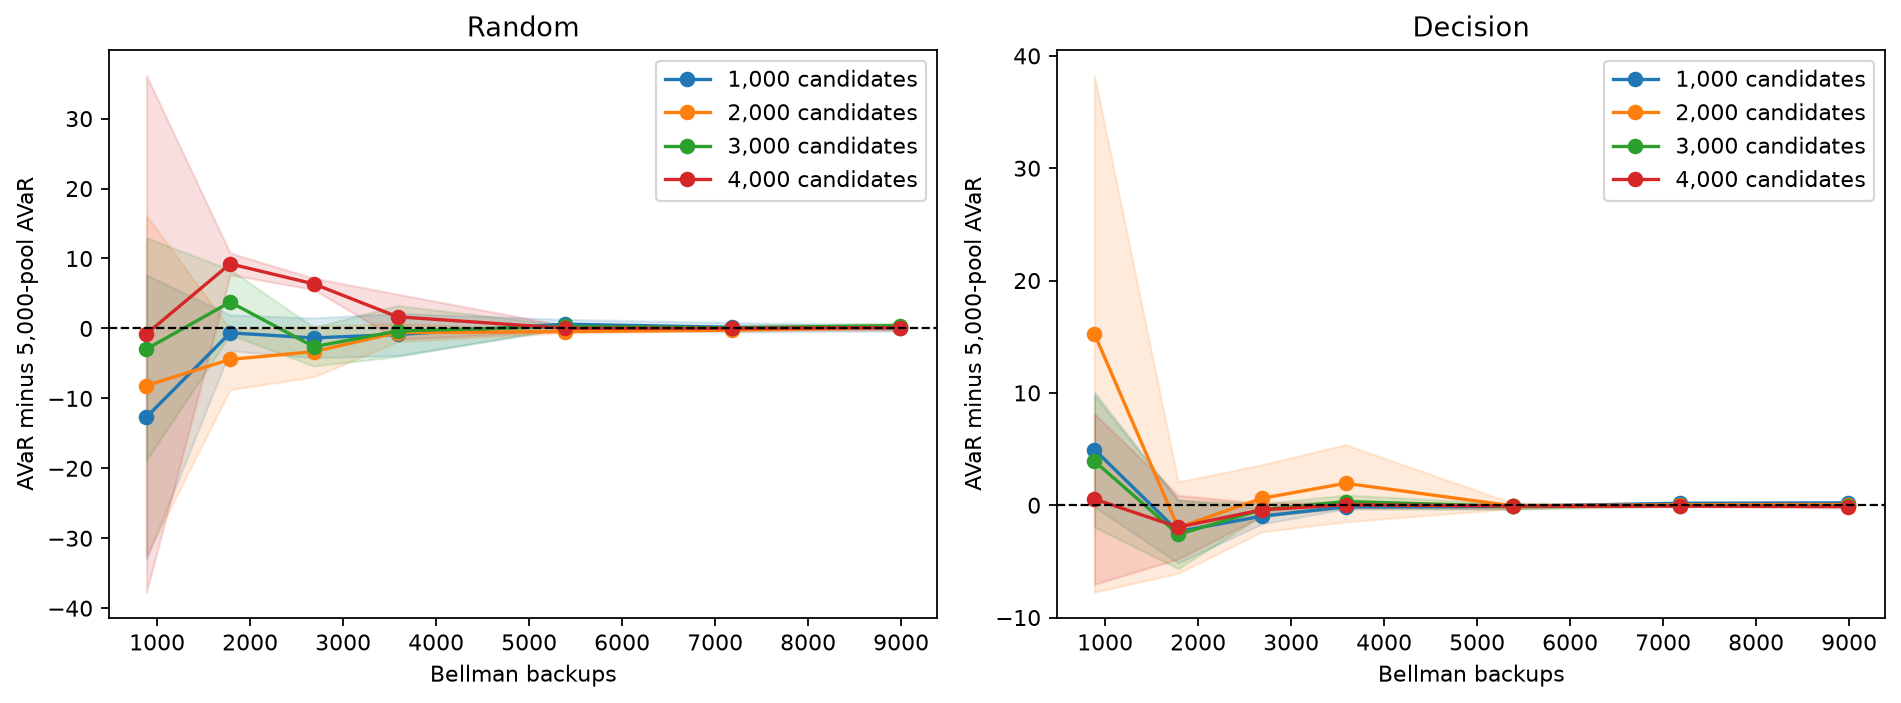
\includegraphics[width=\linewidth]{figures/03_candidate_pool/t7/avar_difference.png}
		\caption{Paired AVaR gaps, $T=7$.}
		\label{fig:pool-paired-t7}
	\end{subfigure}
	
	\caption{Paired AVaR gaps relative to 5{,}000 candidates. Shading shows training-seed standard deviations.}
	\label{fig:pool-paired}
\end{figure}

\paragraph{Pool utilization and increasing budgets.}

More backups do not always improve the policy. For $T=3$, decision-aware AVaR with 1,000 candidates increases from $18.9099$ at 897 backups to $19.5854$ at 5,397 backups. With 5,000 candidates, the increase is smaller, from $18.8852$ to $18.9144$.

At 5,397 backups, the algorithm uses 899 states per stage, corresponding to $89.9\%$ of the smaller pool but only $17.98\%$ of the larger one. High pool utilization leaves less freedom for acquisition, which may contribute to the deterioration.

However, the experiment does not establish its cause. GP refitting and backward propagation of approximate Bellman targets may also contribute. Even with 5,000 candidates, AVaR rises to $19.0388$ at 8,997 backups. Thus, larger pools reduce but do not eliminate the observed deterioration.

Using fewer backups or larger pools may help, but neither guarantees better performance.

\paragraph{Computational trade-off.}

Larger pools increase acquisition costs. At 3,600 nominal backups, increasing the pool from 1,000 to 5,000 candidates raises mean training time from 192 to 257 seconds for $T=3$, and from 68 to 82 seconds for $T=7$, without changing the number of backups.

Candidate-pool size is therefore an additional computational parameter that should be considered together with the Bellman-backup budget.


\subsection{Discussion}
\label{res:discussion}

The main finding is that decision-aware sampling often achieves better policy performance per Bellman backup than random or uncertainty sampling, especially at moderate budgets. Adding reachability or tail weighting does not consistently improve these results.

\paragraph{Value accuracy and policy quality.}

The baseline ADP achieves policy performance close to exact DP despite noticeable root-value errors. This shows that accurate value estimation and accurate action selection are different objectives. As shown by the action-gap result in Section~\ref{theory:action-gap}, approximation errors may preserve the optimal action when they are sufficiently small relative to the true action gap. The experiments are consistent with this result but do not verify the condition at every state.

Outer-threshold optimization additionally depends on the accuracy of the predicted RU objective. A good fixed-threshold policy or a small predicted objective does not guarantee a good selected threshold. The experiments also do not establish that outer optimization improves on fixed-threshold training, since their configurations and budget allocations differ.

\paragraph{Paired evaluation.}

Paired evaluation reduces Monte Carlo noise when comparing policies. For $T=3$, much of the difference from the exact AVaR comes from the finite evaluation sample. However, pairing does not remove actual policy differences or sampling uncertainty.

All training seeds use the same evaluation trajectories, so averaging over seeds does not remove sampling error. Also, empirical AVaR and fixed-threshold RU may rank policies differently because only AVaR minimizes over the threshold.

\paragraph{Reachability and tail weighting.}

The additional scores use trajectories generated by the fitted risk-neutral policy, which may not represent the states important under the AVaR policy. Multiplying these scores by decision uncertainty may also reduce the priority of useful states. Furthermore, threshold exceedance is only a proxy for the effect of action errors on AVaR.

These are possible explanations for the mixed results. Experiments on tail relevance weighting did not show meaningful improvements either. Thus, better ways of incorporating reachability and tail relevance might be a subject for further research.

\paragraph{Candidate pools and computational cost.}

The candidate-pool experiment shows that more Bellman backups do not always improve policy performance. Smaller pools can restrict acquisition when most candidates are already selected. Larger pools reduce the observed deterioration for $T=3$, but do not guarantee improvement. GP refitting and backward propagation of approximation errors may also contribute, although their effects were not isolated.

Backup efficiency also differs from runtime efficiency. Repeated GP fitting and acquisition calculations can make decision-aware sampling slower than random sampling. However, decision-only acquisition avoids the additional rollouts and nearest-neighbor calculations required for reachability and tail scores. Its accuracy and simpler acquisition procedure make it attractive, although the experiments do not establish a consistent accuracy-runtime advantage over the weighted variants.

\paragraph{Further threshold-search improvements.}

The same trained GP models can evaluate the predicted RU objective at different thresholds. An adaptive search could therefore reduce root evaluations and leave more budget for GP training. However, the optimized RU objective is not necessarily convex or unimodal, so local optimization does not guarantee a global minimum.

\paragraph{Limitations.}

The experiments consider one scalar control problem, two horizons, and one confidence level. Exact DP is available only for $T=3$ under discretized disturbances, and its threshold is grid-optimal. For $T=7$, the fixed threshold is heuristic, and its pilot estimation shares an evaluation seed with later benchmarks.

Baseline evaluation may randomly initialize and cache unseen states. Evaluation-order dependence was confirmed for the saved $T=7$ policy, but its effect on benchmark rankings was not established. Baseline comparisons and their Monte Carlo intervals therefore require caution.

GP uncertainty is model-based and does not guarantee small Bellman approximation errors. The risk-neutral continuation is also approximated, despite the exact mathematical decomposition for $y\geq0$. Finally, some experiments use only three training seeds, and shared evaluation trajectories introduce common Monte Carlo uncertainty.

Thus, the results support decision-aware Bellman allocation within the tested settings, without establishing general superiority or convergence. The main remaining question is how reachability and tail information can improve policy accuracy beyond decision uncertainty alone.
